\chapter*{Практика 5. OFDM модуляция}
\addcontentsline{toc}{chapter}{Практика 5. OFDM модуляция}
\label{ch:5_practice}

\textit{\textbf{Задание:}} Реализовать OFDM модулятор.

\begin{itemize}
    \item Разработан OFDM модулятор со следующими компонентами:
    \begin{itemize}
        \item Вставка пилотных символов
        \item Добавление нулевых поднесущих (25\%)
        \item Применение ОБПФ
        \item Добавление циклического префикса
        \item Сохранение параметров модуляции для демодулятора
    \end{itemize}
\end{itemize}

\begin{figure}[ht]
    \centering
    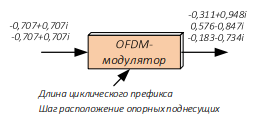
\includegraphics[width=0.8\textwidth]{ofdm_modulator.png}
    \caption{Структура OFDM модулятора}
    \label{fig:ofdm_modulator}
\end{figure}

\begin{figure}[ht]
    \centering
    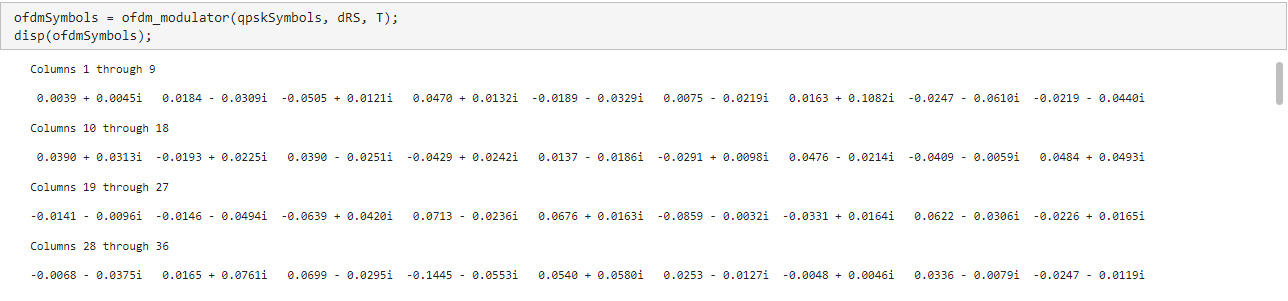
\includegraphics[width=0.8\textwidth]{5practice_result.png}
    \caption{Результат пятой практики}
    \label{fig:5practice_result}
\end{figure}